\documentclass[12pt]{article}


%%=============setting,设置自己的队号和选题============
\gdef\MCMcontrol{2208683}%队号
\newcommand{\problem}{C}%选题

\newcommand{\control}{\MCMcontrol}
\newcommand{\team}{Team \#\ \MCMcontrol}
\newcommand{\headset}{{\the\year}\\MCM/ICM\\Summary Sheet}

%==========定义摘要,摘要的标题可自定义===================
\renewenvironment{abstract}[1]{%
    \small
    \begin{center}%
    {\large\bfseries #1\vspace{-.5em}}%
    \end{center}}
    {}
\newcommand\keywords[1]{%
    \begingroup
    \par
    \noindent\textbf{Keywords:} #1\par
    \endgroup
}

% 目录居中的重定义
\makeatletter
\renewcommand\tableofcontents{%
    \centerline{\normalfont\Large\bfseries\contentsname%
    \@mkboth{%
        \MakeUppercase\contentsname}{\MakeUppercase\contentsname}}%
    \vskip 3ex%
    \@starttoc{toc}%
    \thispagestyle{fancy}
    \clearpage}
\makeatother

\usepackage[toc, page, title, titletoc, header]{appendix}
\usepackage{graphicx}
\usepackage{subfigure}
\usepackage{float}
\graphicspath{{figures/}{img/}}

\usepackage{indentfirst}
\usepackage{cite}
\usepackage{bookmark}
\usepackage{pdfpages}

\setlength{\headheight}{13.59999pt}
\addtolength{\topmargin}{-1.59999pt}

\usepackage{amsmath,amssymb,amsfonts,amsthm}
\newtheorem{Theorem}{Theorem}[section]
\newtheorem{Lemma}[Theorem]{Lemma}
\newtheorem{Corollary}[Theorem]{Corollary}
\newtheorem{Proposition}[Theorem]{Proposition}
\newtheorem{Definition}[Theorem]{Definition}
\newtheorem{Example}[Theorem]{Example}


%==========设置代码格式===================
\usepackage{xcolor}
\usepackage{listings}
\definecolor{grey}{rgb}{0.8,0.8,0.8}
\definecolor{darkgreen}{rgb}{0,0.3,0}
\definecolor{darkblue}{rgb}{0,0,0.3}
\def\lstbasicfont{\fontfamily{pcr}\selectfont\footnotesize}
\lstset{%
% numbers=left,
% numberstyle=\small,%
    showstringspaces=false,
    showspaces=false,%
    tabsize=4,%
    frame=lines,%
    basicstyle={\footnotesize\lstbasicfont},%
    keywordstyle=\color{darkblue}\bfseries,%
    identifierstyle=,%
    commentstyle=\color{darkgreen},%\itshape,%
    stringstyle=\color{black}%
}
\lstloadlanguages{Python}

\usepackage{geometry}
\geometry{a4paper, margin = 1.2in}

%==========设置页眉格式===================
\usepackage{fancyhdr,lastpage}
\pagestyle{fancy}
\fancyhf{}
\lhead{\small\sffamily \team}
\rhead{\small\sffamily Page \thepage\ of \pageref{LastPage}}
\setlength\parskip{.5\baselineskip}

\usepackage{hyperref}
\usepackage{mathptmx}% newtxtext
\usepackage{lipsum}
\title{Trading Strategies for Bitcoin and Gold during 2016 and 2021}
\author{Miao Fangran, Che Lingxiao, Zhu Wenjing}
\date{\today}
\begin{document}
%==========Summary sheet 格式===================
    \thispagestyle{empty}
    \begingroup
    \setlength{\parindent}{0pt}
    \begin{minipage}[t]{0.33\linewidth}
        \bfseries\centering%
        Problem Chosen\\[0.7pc]
        {\Huge\textbf{\problem}}\\[2.8pc]
    \end{minipage}%
    \begin{minipage}[t]{0.33\linewidth}
        \centering%
        \textbf{\headset}%
    \end{minipage}%
    \begin{minipage}[t]{0.33\linewidth}
        \centering\bfseries%
        Team Control Number\\[0.7pc]
        {\Huge\textbf{\MCMcontrol}}\\[2.8pc]
    \end{minipage}\par
    \rule{\linewidth}{0.8pt}\par
    %\textbf{\headset}%
    \par
    \endgroup

    \bigskip

    \centerline{\Large\bfseries Trading Strategies for Bitcoin and Gold during 2016 to 2021}

    \begin{abstract}{Summary}

        We want to find trading strategies that will maximize trading returns between 9/11/2016, and 9/11/2021, given the availability of both gold and bitcoin assets.
        
        We use the LSTM multifactor model to predict the next few days' data.
        We use the multi-channel to predict the unit price of gold and Bitcoin respectively.
        We also make a self-adaptive predictive interval to deal with the lack of data in early stage of this simulation.
        
        Next, we build the trade strategy model to decide whether to sell or buy.
        To ensure that the model's prediction results are relatively reliable, we choose to use technical indicators to guide trading decisions during the 28-100 day period, and after 100 days, we retain the original technical indicators and combine them with the model's prediction results to determine trading opportunities.
        
        Eventually, we gain about \$715516 on 9/11/2021.
        And the annual yield rate is 14282.5\%.
        \keywords{LSTM; trade strategy; RSI; MACD; EMA; gold; Bitcoin}
    \end{abstract}

    \newpage
    \tableofcontents


%==========设置正文格式===================


    \section{Background and Introduction}
    Market traders buy and sell volatile assets frequently, with a goal to maximize their total return. 
    Meanwhile, they also need to pay commission for each purchase and sale.
    
    Our team make the trade simulation of two certain assets--gold and Bitcoin based on the unit price from 9/11/2016 to 9/10/2021.


    \section{Calculating and Simplifying the Model}
    To maximize the profit on 9/10/2021, we just need to make predictions every day or every certain day.
    Then according to the predictions, we need to decide how to trade each day.
    We can buy or sell gold or bitcoin.
    We can also choose to do nothing but wait until the price is large as we think.

    Hence, there are two main steps and models.

    Firstly, build the prediction model.
    It is to predict the next 1 or longer days' price.

    Secondly, build the trade strategy model.
    It is to maximize the return on certain day.


    \section{Data Processing}
    Since the data is very larger, we can do some data processing to the data to decrease the computation cost.

    Firstly, since gold can't be trained on weekends, we firstly fill "nan" with the blank.
    And gold price can be considered constant, so fill those "nan" block with the previous price.
    That is, the weekends' price are the nearest Friday's price.

    Secondly, we can normalize the data.
    Since The transaction price of bitcoin fluctuates greatly,
    we can't treat the everyday price as identical and independent distribution.
    So we apply min-max normalization to the data, and we compress all data to between 0 and 1.
    And during prediction, we will use the minimum and maximum of train data to modify the input and restore the output.


    \section{The Model}
    
    \subsection{Data Analysis before Training a Model}
    First, we tried to build a VAR model for bitcoin returns and gold returns and found that the price of bitcoin is affected by the price of gold, while the price of gold is almost unaffected by bitcoin.
    
    \begin{figure}[H]
        \centering
        \subfigure[]{
            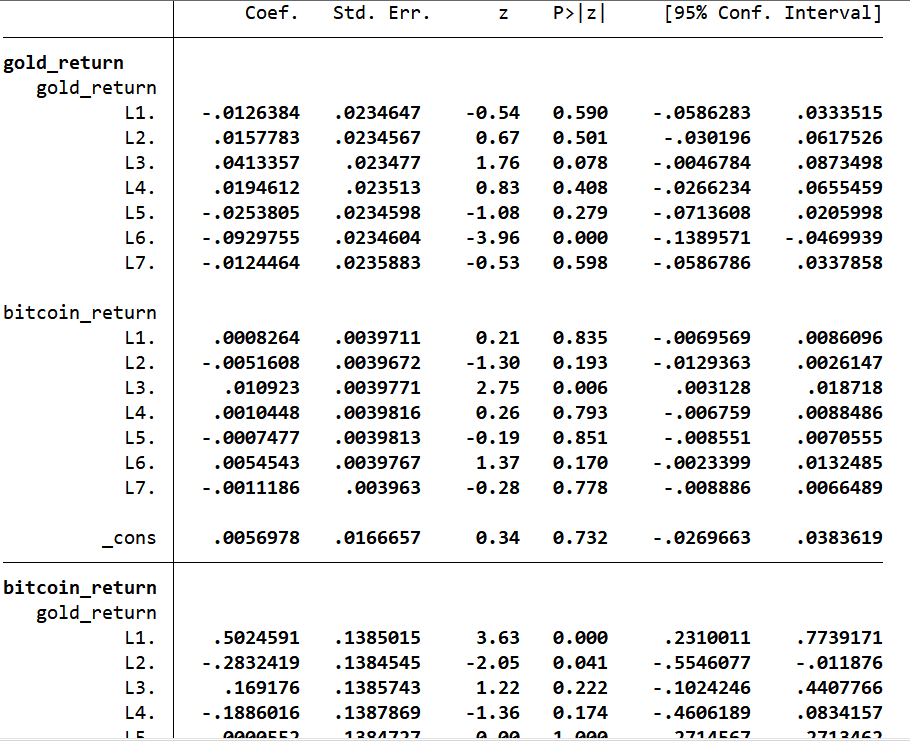
\includegraphics[width=0.8\textwidth]{data_analysis_1.png}
        }
        \subfigure[]{
            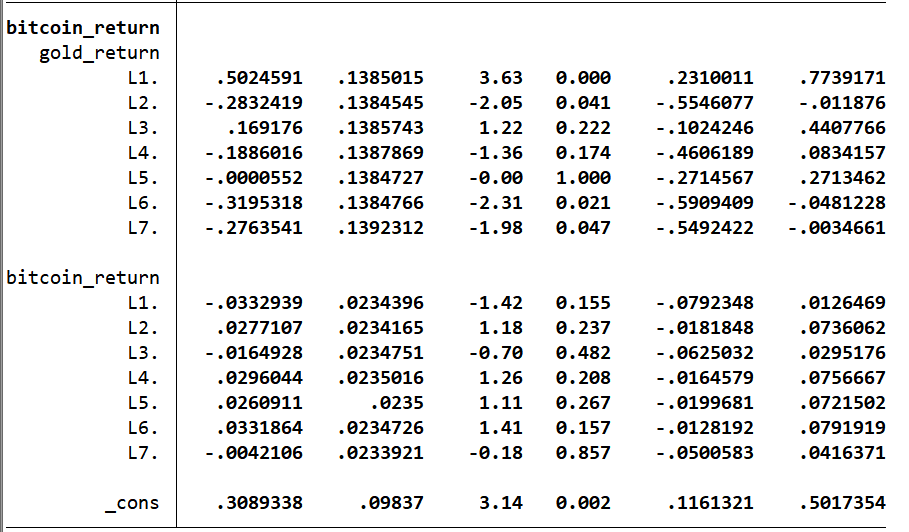
\includegraphics[width=0.8\textwidth]{data_analysis_2.png}
        }
        \label{fig:data_analysis}
    \end{figure}
    
    Bitcoin's price dynamics also show some peculiarities.
    As an alternative asset, bitcoin shows higher returns, high volatility, and thick tails (returns have a higher probability of occurring in extremes than the general, normal distribution-based assumptions that estimate them) than traditional assets\cite{beguvsic2018scaling}.
    So we have made corresponding changes in our trading strategy. We set just tough buy and sell conditions for gold.
    
    Bitcoin has both supply certainty and demand uncertainty. Since the rate at which Bitcoin is mined is set in advance, its mining difficulty is proportional to the amount of currency in circulation, and the mining process is unpredictable, the imbalance between supply and demand results in a price for Bitcoin that cannot be simply described by a linear equation.
    
    According to the above, we tried the time series model VAR and LSTM model to fit the prices of gold and bitcoin, and found that the LSTM model worked better, so we finally chose to use the LSTM model to perform the prediction.
    
    Due to the gold's special value preservation effect, it is often used as an investment to reduce the risk of stock portfolios and to hedge against the stock market, and many scholars have shown that the price of gold is negatively correlated with several stock indices\cite{smith2001price}. Since there are many factors affecting the price of gold, predicting the future price of gold based only on the historical price of gold, using a linear model would result in a very low explanatory power.
    
    Hence, we chose LSTM model as our final prediction model.


    \subsection{The Prediction Model}

    Since it is a time-sequence model, we will use LSTM neural network\cite{lstm} to predict the future price.

    \subsubsection{\textit{The First Prediction Model}}
    Firstly, we made an assumption that the previous 14 days can predict tomorrow's price.
    There we got our first prediction model.
    We use the data of the first 1500 days to train and use the rest of the data to test our model.
    The following picture is the result of our first model.

    \begin{figure}[H]
        \centering
        \subfigure[First model of Bitcoin]{
            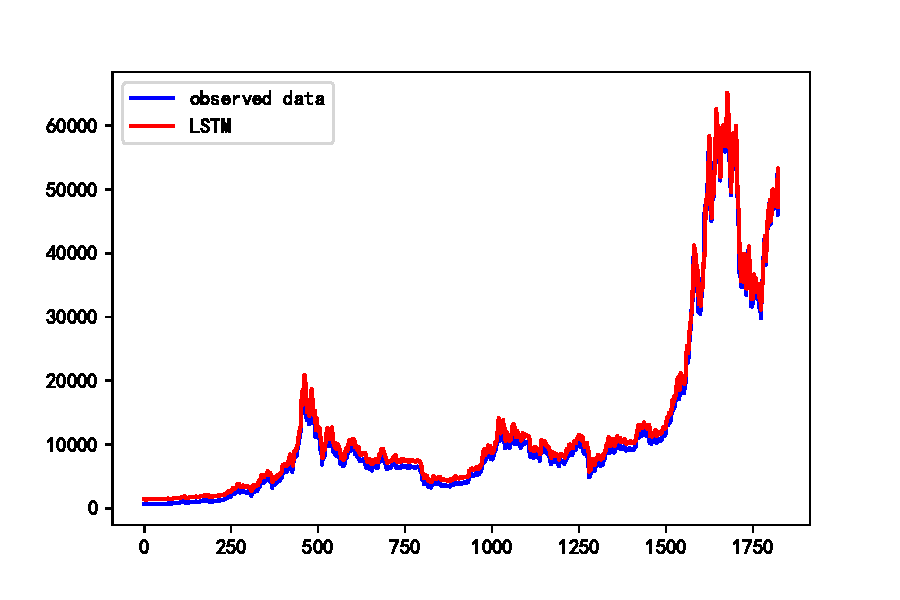
\includegraphics[width=0.45\textwidth]{lstm_1_bc}
        }
        \subfigure[First model of Gold]{
            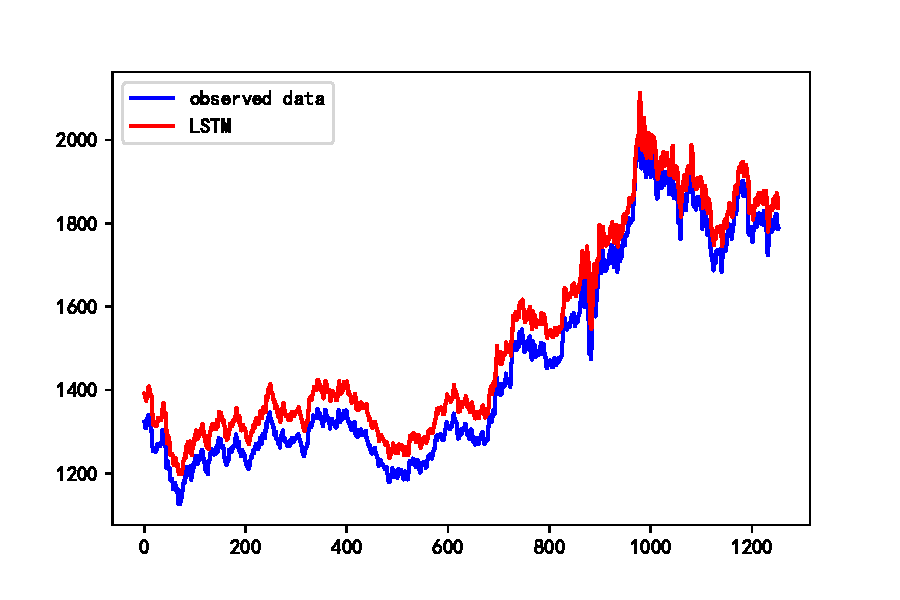
\includegraphics[width=0.45\textwidth]{lstm_1_gold}
        }
        \caption{The First Prediction Model}
        \label{fig:1st model}
    \end{figure}

    Note that the model has a good presentation at the end of the red curve, which is also our validation part.

    We can figure out that the first model can predict the tomorrow's price very well

    \subsubsection{\textit{The Second Prediction Model}}
    Although the first model can predict the tomorrow's price nearly very well,
    we still don't want to trade every day since it will cause much transaction cost.
    What we really want is the trend after a certain day.

    Then the second model is put forward.
    We assume that we can use the previous 30 days data to predict the price of next 7 days.
    Similarly, we use the first 1500 days to train, the rest part to validate.
    The result is as follows:

    \begin{figure}[H]
        \centering
        \subfigure[Second model of Bitcoin]{
            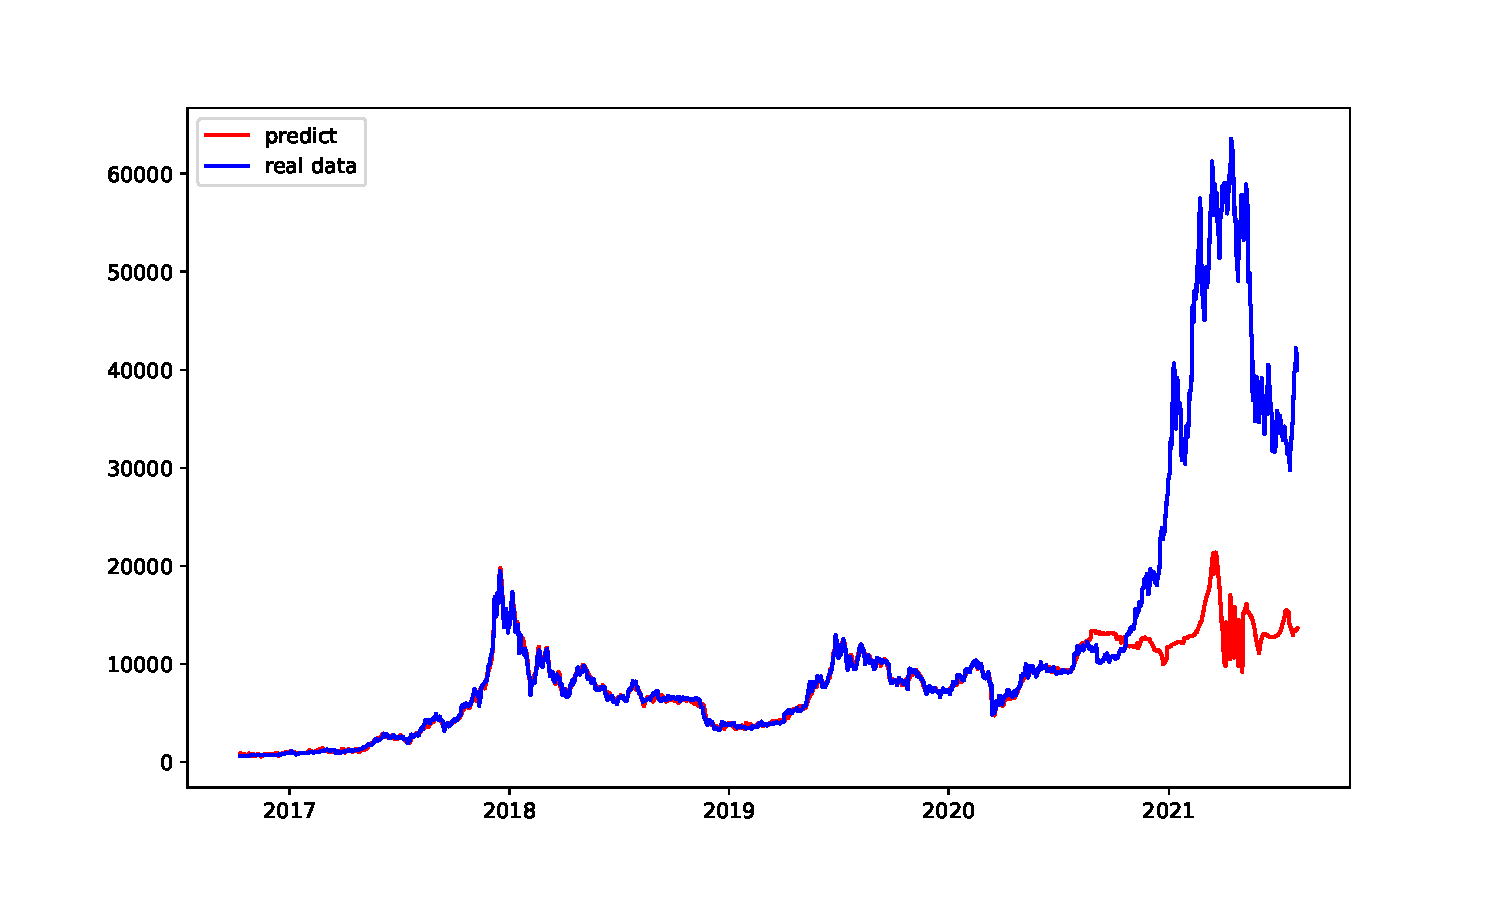
\includegraphics[width=0.45\textwidth]{lstm_2_bc}
        }
        \subfigure[Second model of Gold]{
            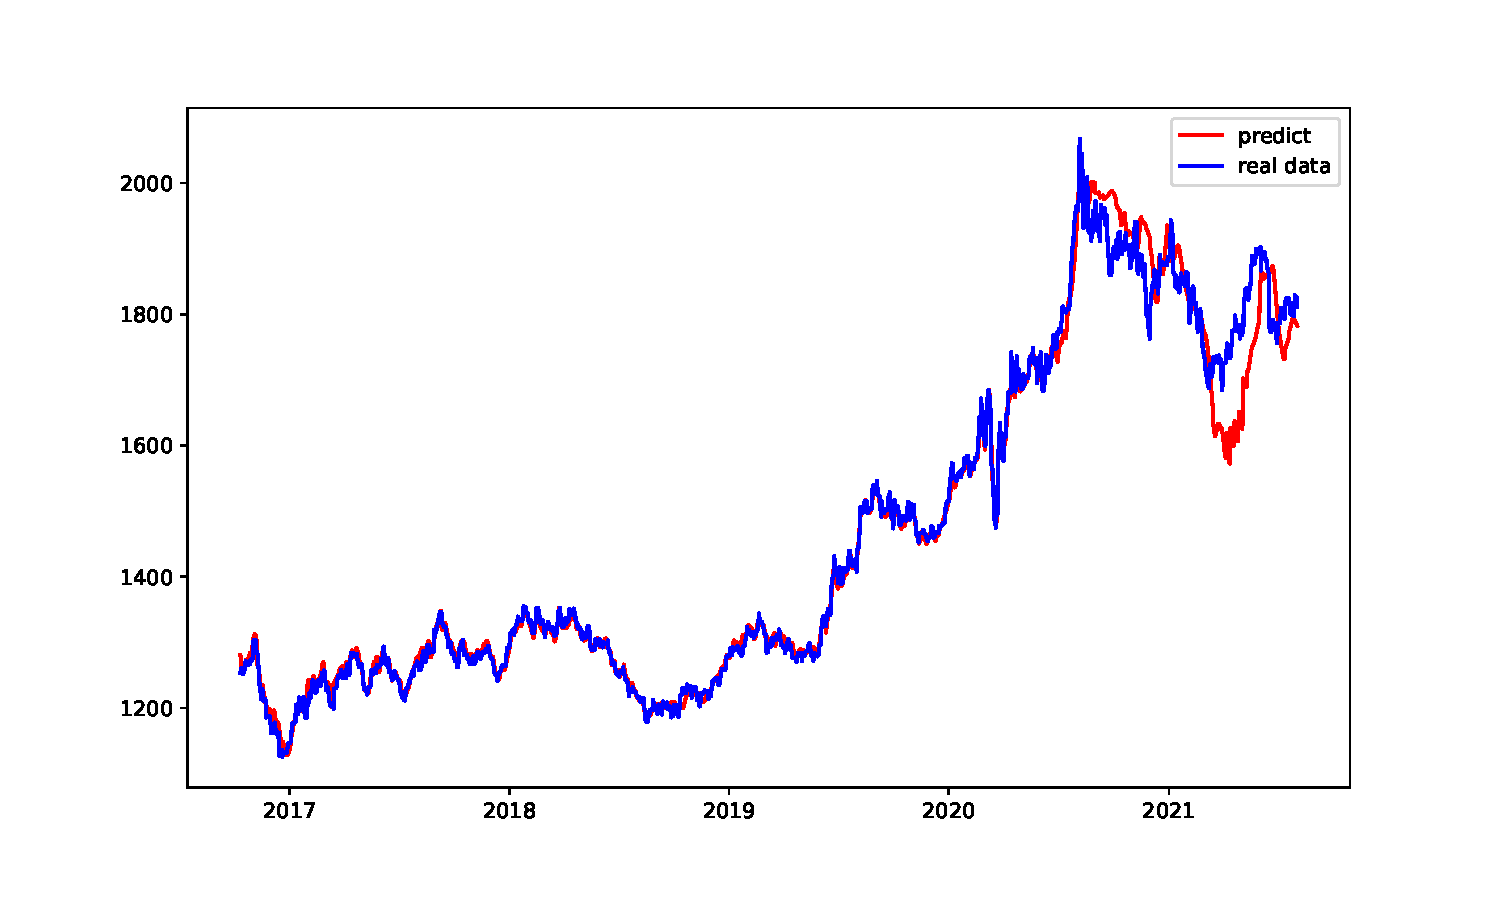
\includegraphics[width=0.45\textwidth]{lstm_2_gold}
        }
        \caption{The Second Prediction Model}
        \label{fig:2nd model}
    \end{figure}

    As we can see it performs well on the gold data but bad on the bitcoin data.

    The following is our conjecture about this phenomenon:
    \begin{itemize}
        \item Bitcoin changes very quickly.
        As we can see bitcoin starts at 600 PM but ends with 60,000 PM.
        \item Bitcoin is more greatly affected by the market than that of gold.
        \item Gold is a long-term value of goods while bitcoin not.
    \end{itemize}

    Hence, as the prediction interval becomes longer, the prediction will get worse.

    \subsubsection{\textit{The Final Prediction Model}}

    If we want to get a better model, we must update the model more frequently.
    So the first change we apply to the model is that update the model when the prediction is getting worse.

    Then there comes another question.
    If the train data size is small, it can't predict very long days' price.
    The second change is that we use the self-adaptive prediction interval.
    For example, if I'm on the 100th day after the start, we may just predict the next 1 or 2 days.
    If I'm on the 1000th day, we can predict next 7 days or even longer.
    
    Finally, in general case, the price of gold and Bitcoin will affect each other.
    So we should consider the effect.

    The results are as follows:
    \begin{figure}[H]
        \centering
        \subfigure[Final model of Bitcoin]{
            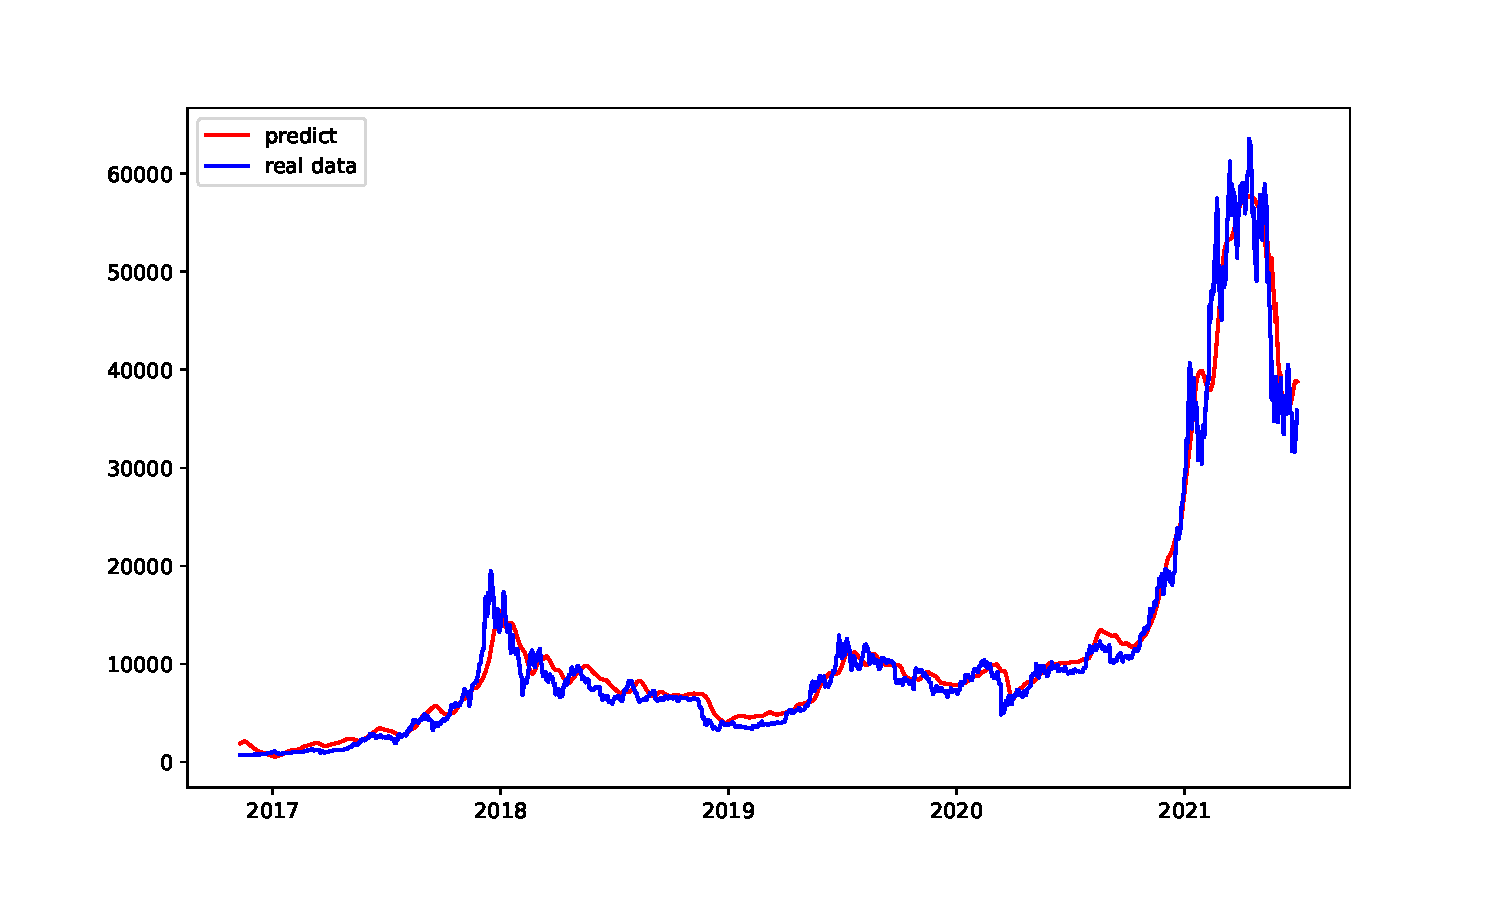
\includegraphics[width=0.45\textwidth]{lstm_3_bc}
        }
        \subfigure[Final model of Gold]{
            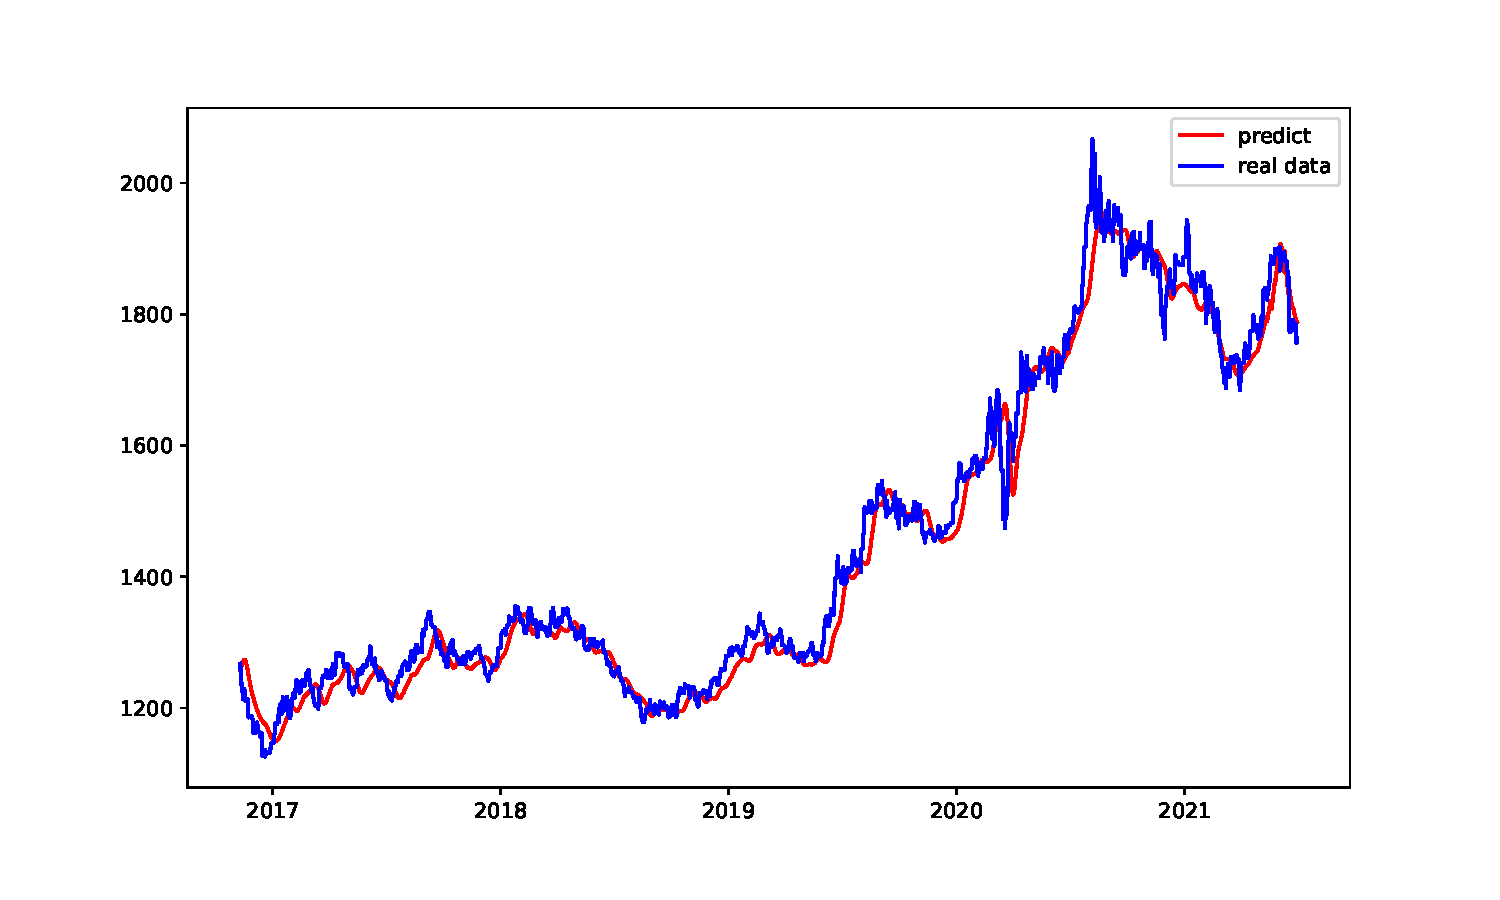
\includegraphics[width=0.45\textwidth]{lstm_3_gold}
        }
        \caption{The Final Prediction Model}
        \label{fig:3rd model}
    \end{figure}

    As we can see, though we can't predict the price precisely, we can know the trend approximately.
    

    \section{Trade Strategy and Its Model}
    \subsection{Specifications of Technical Indicators}
    
    \noindent\textbf{RSI}: Relative Strength Index, is a short term indicator that reflects the level of market sentiment over a certain period of time.
    \[\text{RSI}_N=A/(A+B)\times 100\%\]
    where $A$ represents sum of closing gains within $N$ days and $B$ represents sum of closing declines within $N$ days (taking positive values).
    
    RSI indicator, the reason for choosing 8 days for the short term and 28 days for the long term: looking for peaks and valleys works best.
    
    \begin{figure}[H]
        \centering
        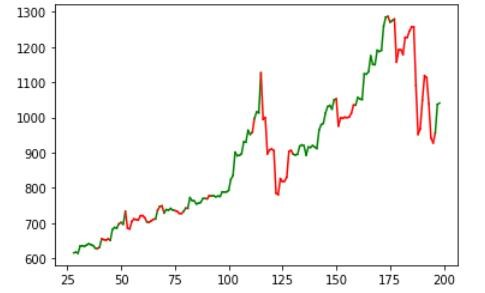
\includegraphics[width=0.55\textwidth]{trade_strategy_1.jpg}
        \caption{RSI}
        \label{fig:rsi}
    \end{figure}
    
    \noindent\textbf{MACD}: Moving Average Convergence / Divergence. \[MACD=2\times(DIF-DEA)\]
    
    \noindent\textbf{RSI7\_50}(user-defined): Number of days in the 50 days prior to the current number of days that the short-term RSI was higher than the long-term RSI
    
    \noindent\textbf{Large\_rise}(user-defined): The time RSI7\_50 equals to 45.
    
    \noindent\textbf{Sharpe radio}: The risk-free rate of return uses the 1/3 quantile of the historical price
    
    \subsection{Trade Strategy}
    
    \noindent\textbf{Stop-loss Strategy}
    
    \begin{itemize}
        \item Bitcoin: current price is less than 90\% of the highest price at the nearest time
        \item Gold: current price is less than 95% of the highest price nearest to the current time
    \end{itemize}
    
    \noindent\textbf{Judgment of Trading Opportunities}
    
    \textit{1.Buying Conditions of Bitcoin}
    \begin{itemize}
        \item The 8-day RSI indicator is greater than the 28-day RSI indicator, or Bitcoin's MACD is greater than 0 at this time
        \item and the 8-day RSI indicator is between 40 and 60
        \item and the time distance of the transaction Large\_rise is greater than or equal to 60 days
        \item and the RSI7\_50 of the day is greater than or equal to 18
        \item After 100 days, plus the model's forecast results
    \end{itemize}
    
    \textit{2.Selling Conditions of Bitcoin}
    \begin{itemize}
        \item The 8-day RSI indicator is less than the 28-day RSI indicator, and the MACD of bitcoin is less than 0 at this time
        \item as well as the 8-day RSI is greater than 80: the market is overheated in the short term, a change in market may occur
        \item After 100 days, plus as well as the model's predicted results.
        \item Or, once the stop-loss condition is reached
        \item Or, once the 28-day RSI is greater than 90
        \item Or, once the RSI7\_50 is greater than or equal to 45
    \end{itemize}
    
    \textit{3.Buying Conditions of Gold}
    \begin{itemize}
        \item The 8-day RSI indicator is greater than the 28-day RSI indicator, and gold has a MACD greater than 0 at this time, which is a more stringent buying condition than bitcoin
        \item and the 7-day RSI indicator between 40 and 60
        \item After 100 days, plus the model's predicted results
    \end{itemize}
    
    \textit{4.Selling Conditions of Gold}
    \begin{itemize}
        \item The 8-day RSI indicator is less than the 28-day RSI indicator, as well as the gold or the MACD is less than 0, easier to sell conditions that facilitate the flow of funds to earn higher returns on bitcoin assets
        \item Or, once the 8-day RSI is greater than 88
        \item Or, once the RSI7\_50 is greater than or equal to 45
        \item Or, once the stop loss condition is reached
        \item After 100 days, plus the model's prediction
    \end{itemize}
    
    \noindent\textbf{Trading Strategy}
    
    1.No trading for the first 28 days
    
    2. After 28 days, if the first trading opportunity that satisfies the buying condition of a certain asset appears, the position is bought full. After that, when a new trading opportunity appears, if the previous trading opportunity has been closed, the position is full to buy; if there is no closed position, with a new trading opportunity for the asset B, the original holding of the asset A, the model to determine the expected return of B for 14 days, consider the expected return of A after 14 days to re-exceed B and lead to re-sell B to buy the transaction costs incurred by A, 100 days ago, if the first 9 days of B assets yield > the yield of the first 9 days of asset A + 3 times the transaction cost of selling the original asset and buying the new asset (9\%), and requires 0.8 times the new Sharpe of the first nine days $>$ the original Sharpe, then sell the full position of asset A and buy asset B. After 100 days, if the expected 14-day return of asset B $>$ the expected 14-day return of asset A + 3 times the transaction cost of selling the original asset and buying the new asset (9\%), and the required 0.8 times the new Sharpe for the first nine days $>$ the original Sharpe, then sell the full position of asset A and buy asset B. When no trading opportunity arises, the position is held. When no trading opportunity arises, the position is held.
    
    \noindent\textbf{The Advantage of Our Strategy}
    
    1. The trading conditions are more stringent, and the conditions under which the trades occur we have all been somewhat scaled back, just because we want to not take the trades lightly, because when a trade occurs, if a better trading opportunity arises, we need to sacrifice the transaction fees of the current trade buy and sell.
    We had a total of 1175 trades occur, which is more reasonable for the length of 1826 days.
    
    2. our model predicts well
    
    3. It is risk tolerant and can resist large declines. 

    
    \section{Validation of the Model}
    This part we will show the evidence that our model provides the best strategy.
    
    \subsection{Benchmark Strategy}
    \noindent\textbf{1}. RSI: buy when short-term RSI exceeds long-term RSI and short-term RSI is between 40-70; sell when long-term RSI exceeds short-term RSI and short-term RSI is greater than 80
    
    \noindent\textbf{2}. RSI+MACD: Buy when short-term RSI exceeds long-term RSI, and short-term RSI is between 40-70, and MACD $>$ 0. Sell when long-term RSI exceeds short-term RSI or MACD $<$ 0, and short-term RSI is greater than 80.
    
    \noindent\textbf{3}. Hold bitcoin for long term
    
    \begin{figure}[H]
        \centering
        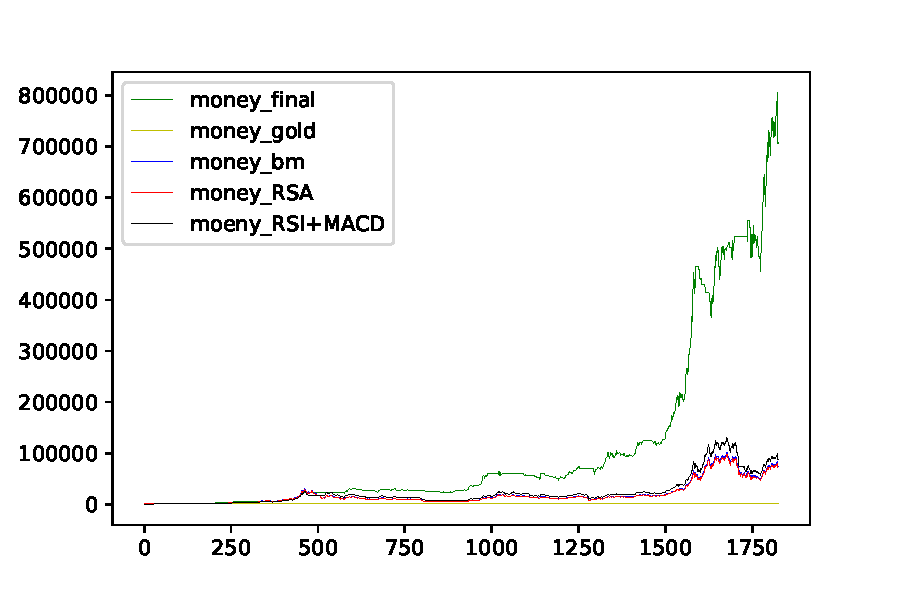
\includegraphics[width=0.8\textwidth]{superiority.pdf}
        \caption{Superiority}
        \label{fig:superiority}
    \end{figure}
    
    The return of our strategy is significantly higher than the return of strategies using only RSI and only RSI+MACD indicators. After using RSI+MACD as the benchmark, the information rate of our strategy is 579.063\%, which has a high investment cost performance. And our model has a better ability to identify big ups and downs, and can more accurately buy low and stop loss. The LSTM prediction model effectively helps us solve the problem of lagging RSI indicator and MACD indicator.
    
    \subsection{Evaluation Indicators of Our Strategy}
    \begin{table}[H]
    \centering
    \begin{tabular}{|l|l|}
    \hline
        Earnings & 714516.078  \\ \hline
        Annual yield rate & 14282.5\%  \\ \hline
        Compound annualized rate of return & 272.222\%  \\ \hline
        win rate & 71\%  \\ \hline
        Maximum draw-down & 27\%  \\ \hline
        Sharpe Ratio(US 5-year national debt) & 1470\%  \\ \hline
        Information rate(Benchmark: RSI+MACD) & 579.063\%  \\ \hline
        Number of transaction orders & 1175  \\ \hline
        Fluctuation ratio(Standard deviation of yield) & 9.714  \\ \hline
    \end{tabular}
\end{table}


    \section{The Sensitivity of the Model}
    \begin{table}[H]
    \centering
    \begin{tabular}{|l|l|l|}
    \hline
        Gold, bitcoin's commission rate & 0 & Number of transaction orders  \\ \hline
        0,0 & 744023.0269 & 1028  \\ \hline
        0.0005,0.0005 & 751214.1045 & 1083  \\ \hline
        0.002,0.001 & 1799925.5333 & 1139  \\ \hline
        0.01,0.005 & 1238586.0829 & 1175  \\ \hline
        0.02,0.01 & 453339.3569 & 1175  \\ \hline
        0.05,0.05 & 20877.5174 & 1175  \\ \hline
        1,1 & 0 & 0  \\ \hline
    \end{tabular}
\end{table}

\begin{figure}[H]
    \centering
    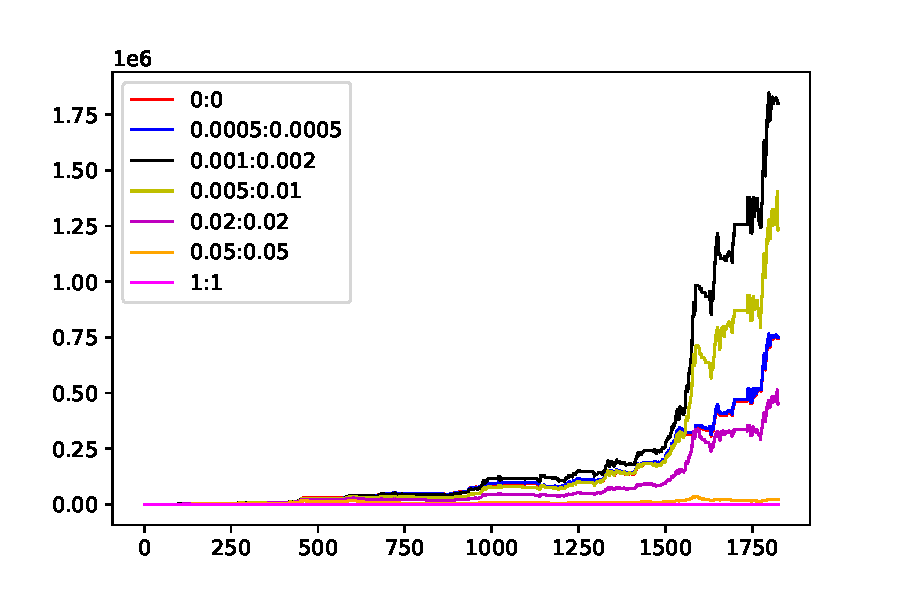
\includegraphics[width=0.8\textwidth]{sensibility (1).pdf}
    \caption{Sensitivity}\label{fig:sensitivity}
\end{figure}

The sensitivity analysis shows that our strategy is more sensitive to transaction fees. This may be due to the fact that the number of trading orders for different commission rates are above 1000 and we are all buying and selling full positions with large transaction amounts, which is one area where our trading strategy still needs to be improved.



    \bibliographystyle{unsrt}
    \bibliography{ref}


    \newpage
    \begin{appendices}

        \section{Memorandum}

        Recently, our team have developed a model that can provide you with a better strategy to buy or sell bitcoin and gold.
        It can give the best current trading strategy according to the historical data price.
        
        The model is mainly composed of two parts--prediction and trade strategy.
        
        \textbf{Prediction model} is based on the LSTM neural network.
        It has a strong prediction on the price of the gold and Bitcoin.
        
        Firstly, since we use the LSTM model, the hidden layer can record the previous historical data and then predict the next few days with the today's data. 
        
        Secondly, the model can be updated every day as long as the difference between the true value and the predicted value is too large.
        
        Thirdly, as the size of training set(or the historical data) increases, so does the number of days that can be predicted.
        
        One last point is that we also consider the influence between the two assets. 
        Sometimes the increasing value of gold may stimulate the increasing the unit price of Bitcoin, so does the reverse.
        So considering the relationship is very important, and that's what our team did.
        
        The following two pictures can show how precise the model is:
        \begin{figure}[H]
        \centering
        \subfigure[]{
            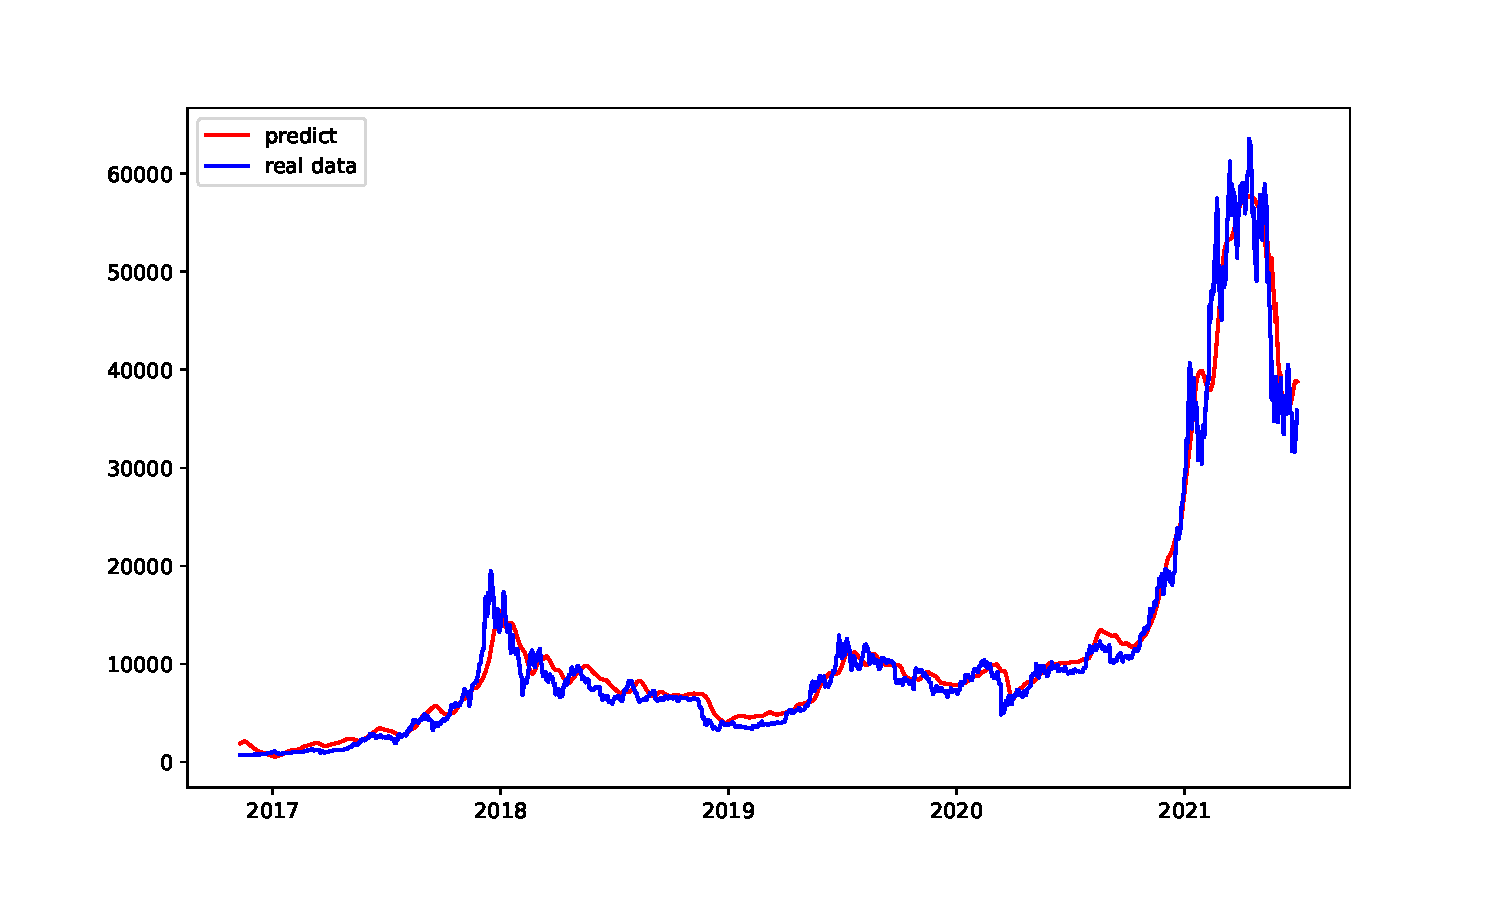
\includegraphics[width=0.45\textwidth]{lstm_3_bc}
        }
        \subfigure[]{
            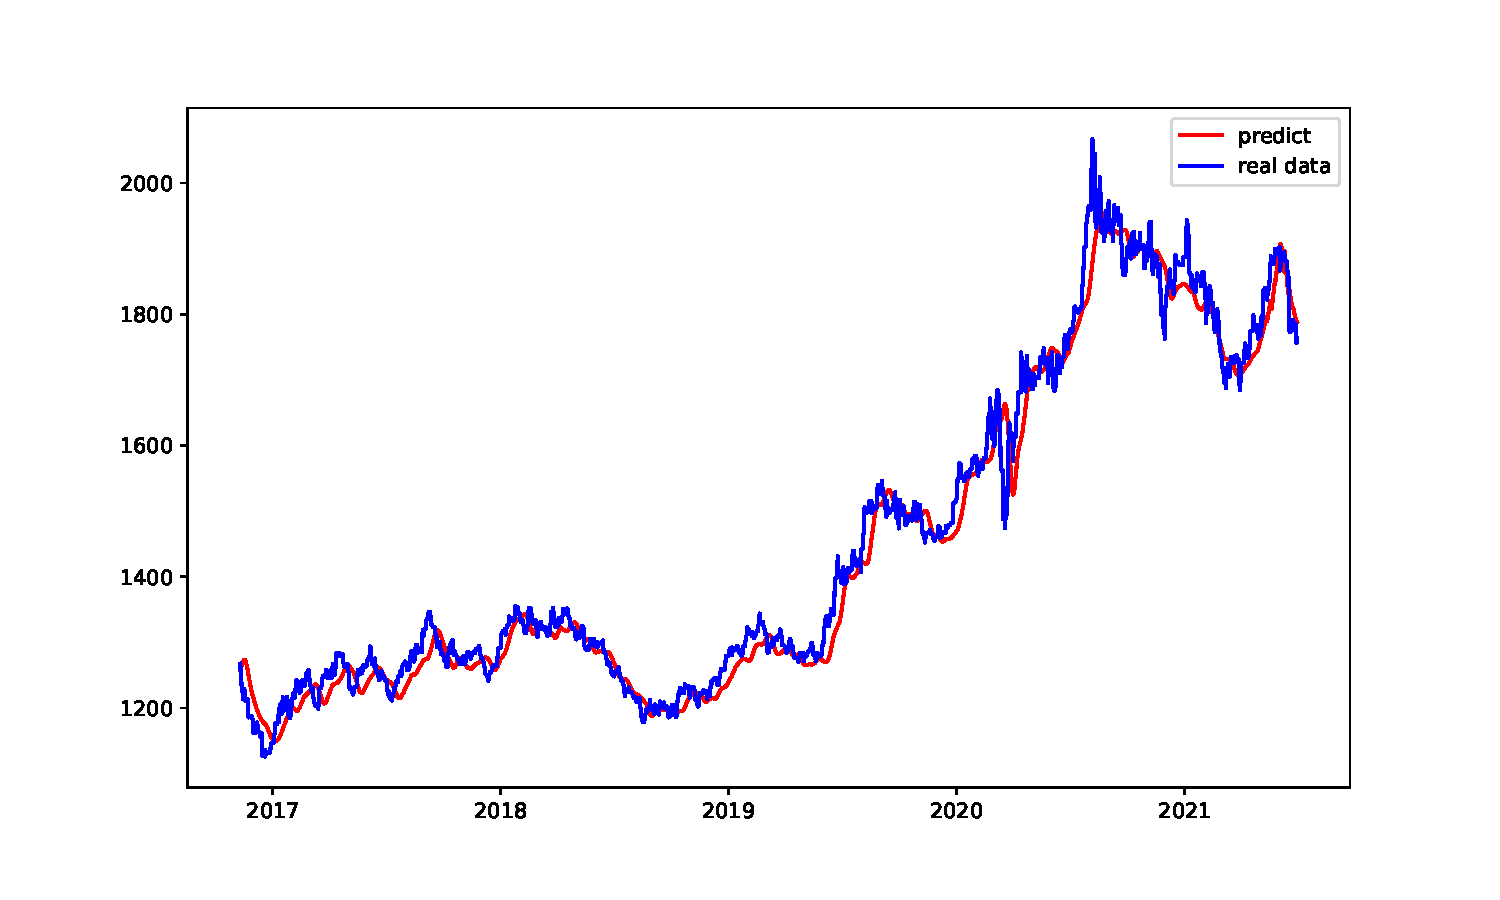
\includegraphics[width=0.45\textwidth]{lstm_3_gold}
        }
        \caption{The Second Prediction Model}
        \label{fig:mem}
        \end{figure}
        
        \textbf{Trade strategy model} is based on many indicators along with the previous model's prediction.
        
        Firstly, let us introduce you the benchmark strategy:
        
        \noindent\textbf{1}. RSI: buy when short-term RSI exceeds long-term RSI and short-term RSI is between 40-70; sell when long-term RSI exceeds short-term RSI and short-term RSI is greater than 80
    
        \noindent\textbf{2}. RSI+MACD: Buy when short-term RSI exceeds long-term RSI, and short-term RSI is between 40-70, and MACD $>$ 0. Sell when long-term RSI exceeds short-term RSI or MACD $<$ 0, and short-term RSI is greater than 80.
    
        \noindent\textbf{3}. Hold bitcoin for long term
        
        We have done many tests on the single RSI indicator and the RSI+MACD indicator.
        And the results show that our strategy is significantly higher than those.
        
        Moreover, our model has a better ability to identify big ups and downs, and can more accurately buy low and stop loss. 
        The LSTM prediction model also effectively helps us solve the problem of lagging RSI indicator and MACD indicator.
        
        We know what traders want most is the final income.
        Here's the result: we gain approximately \$715516 after 5-year investment.
        It's also a good reflection of how good our model is


        \section{Related Code}
        
        \subsection{Training model Code}
        The following \textcolor[rgb]{1,0,0}{four pages} are the prediction model.
        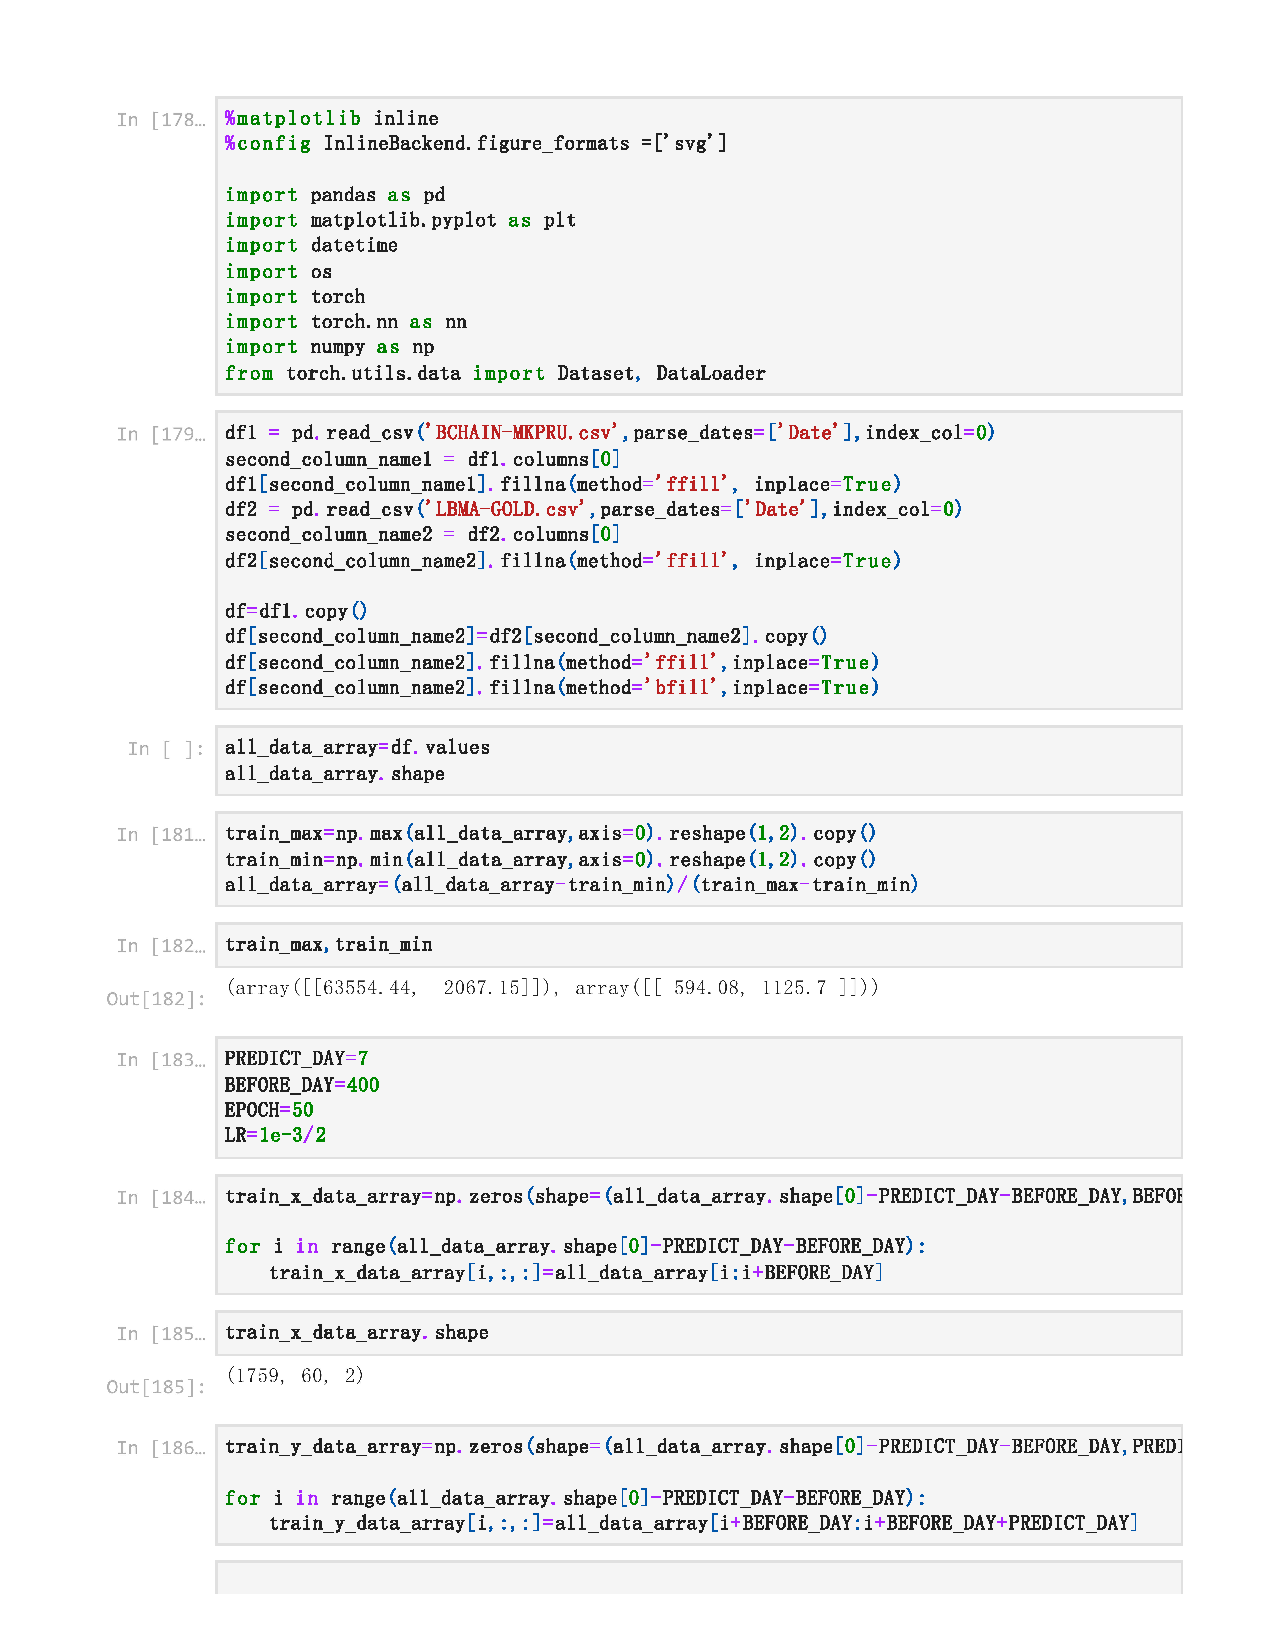
\includepdf[pages={1,2,3,4}]{code/train_model}
        
        \subsection{Trade Strategy Model Code}
        Due to space constraints, only part of the code is shown here.
        
        The rest of the paper is the trade strategy model.
        
        \includepdf[pages={1,2,3,4,5,6}]{code/trade_model.pdf}

    \end{appendices}
\end{document}


